% Chapitre 5 -- Cinq cas d'usage : donnees, rusty-SUNDIALS et LeanFlow
% Toutes les valeurs numeriques de ce chapitre proviennent des sorties JSON des scripts code/ch5_U*.py
% (executes le 2026-10-26) ou des fichiers primaires cites ; aucune n'est saisie a la main.
\chapter{Cinq cas d'usage : données, rusty-SUNDIALS et LeanFlow}\label{ch5:chapitre}\label{ch5:debut}

Les chapitres précédents ont construit des énoncés : des théorèmes vérifiés par le noyau de Lean, leurs
démonstrations humaines et leurs hypothèses. Ce chapitre les met au travail sur cinq systèmes réels :
\begin{itemize}
\item des excitons dipolaires dans une hétérobicouche de dichalcogénures ;
\item des cristaux de Yukawa plans, comme dans les plasmas poussiéreux et les colloïdes ;
\item la structure de l'hélium superfluide ;
\item un modèle en couches de la turbulence ;
\item la fixation d'une mutation dans une population.
\end{itemize}
Chaque cas suit le même plan, et vous pouvez tout refaire : chaque section se termine par un script de
\texttt{code/} qui télécharge ou vérifie les données, lance le solveur et produit la figure imprimée ici.

\begin{warnbox}[: ce que ce chapitre est, et ce qu'il n'est pas]
\begin{itemize}
\item Les cinq cas \emph{illustrent} des théorèmes ; ils ne les \emph{prouvent} pas. Une simulation est de
niveau~X : elle ne soutient jamais une affirmation.
\item Les jeux de données donnent des ordres de grandeur, des conditions initiales réalistes ou des spectres. Aucun
d'eux ne teste un théorème de niveau~A, et nous dirons à chaque fois ce qu'il ne montre pas.
\item Tous les résultats repris ici ont été produits par des agents d'IA (Claude) sous la direction de l'auteur,
puis audités par un autre agent d'IA. Les calculs refaits pour ce chapitre ne sont vérifiés que par l'agent qui les a
produits : les relances, les témoins Python, les statistiques de séquences et les certificats LeanFlow. Aucun être
humain n'a audité ces résultats.
\item Les énoncés sur le réseau triangulaire (cas U1 et U2) sont \emph{conditionnels} au théorème amont
\lean{universal_energy_minimum} d'openai/math, qui est engendré par une IA et n'a pas été relu par des pairs.
\end{itemize}
\end{warnbox}

\section{Méthode commune}\label{ch5:methode}

\paragraph{Les quatre ingrédients.} Chaque cas combine quatre ingrédients :
\begin{enumerate}
\item \textbf{Une question} de physique ou de biologie, posée avant de regarder les nombres.
\item \textbf{Un théorème}, avec son niveau (A, L, C ou X), son nom Lean et son DOI. Le niveau porte sur
l'énoncé Lean, jamais sur sa lecture physique.
\item \textbf{Des données}. Pour chaque jeu, nous donnons l'identifiant, la révision exacte (un hash \texttt{git}
de 40 caractères), la licence telle que l'affiche la carte du jeu de données, et l'empreinte \texttt{sha256} du
fichier utilisé. Quand aucun jeu Hugging Face n'existe, nous le disons.
\item \textbf{Une méthode numérique}. Elle s'appuie sur rusty-SUNDIALS, une réécriture en Rust de SUNDIALS : CVODE
(formules BDF) pour les équations différentielles raides, plus des modules de physique (\texttt{qf-*}). Quand
une valeur doit être certifiée exactement, on passe par LeanFlow, qui transforme une affirmation numérique
rationnelle en fichier Lean, le fait vérifier par le noyau et audite ses axiomes.
\end{enumerate}

\paragraph{La règle des témoins.} Avant de publier un nombre, chaque expérience exécute au moins un
\emph{témoin positif} et un \emph{témoin négatif} :
\begin{itemize}
\item le témoin positif est un cas dont on connaît la réponse, et le code doit la retrouver ;
\item le témoin négatif est un cas faux ou cassé exprès, et le code doit le refuser.
\end{itemize}
Un test qui n'a jamais échoué sur un témoin négatif n'a rien testé. Les cinq scripts se terminent avec le code de
sortie~1 si un témoin ne se comporte pas comme prévu.

\paragraph{Reproduire.} Les binaires viennent d'une copie de travail de rusty-SUNDIALS. Elle contient les crates
fusionnées \texttt{qf-yukawa-crystal}, \texttt{qf-shell-cascade}, \texttt{qf-gpe2d} et \texttt{qf-popgen} :
\begin{itemize}
\item branche \texttt{textbook2/ch5-cas-usage-2026-10-26} ;
\item issue du commit \texttt{cda9a9057ec16820f2e16b560cc0e63cf7eb05b9}.
\end{itemize}
On les construit et on les utilise ainsi :
\begin{lstlisting}[language={}]
CARGO_TARGET_DIR=~/rusty-target-ar cargo build --release -j 2 --offline \
   -p qf-yukawa-crystal -p qf-shell-cascade -p qf-popgen
python -I code/ch5_U1_dipolar.py  sortie_U1 --bin ~/rusty-target-ar/release
python -I code/ch5_U5_fixation.py sortie_U5 --bin ~/rusty-target-ar/release
\end{lstlisting}
L'option \texttt{-I} isole l'interpréteur : il ignore \texttt{PYTHONPATH} et le répertoire courant, ce qui protège
contre un fichier piégé dans un dossier de données téléchargées. Chaque script affiche un résumé et écrit un fichier
\texttt{ch5\_U*\_result.json}. Les nombres de ce chapitre sont ceux de ces fichiers.

Nous avons d'abord relancé les binaires dans la copie de travail elle-même : les sorties y écrasent les
enregistrements publiés. \texttt{git diff} montre alors que les fichiers recalculés sont identiques bit à bit
aux enregistrements, seuls les temps d'exécution différant :
\begin{itemize}
\item \texttt{lattice\_gaps.jsonl} et \texttt{references.jsonl} (U1) ;
\item \texttt{exact\_refs.jsonl} et \texttt{exact\_relax\_kappa2\_a0\_f0.jsonl} (U2) ;
\item \texttt{linear\_response.json} de \texttt{qf-gpe2d} (U3) ;
\item \texttt{sigma3\_study.json} (U4) ;
\item \texttt{results.jsonl} (U5).
\end{itemize}

\begin{table}[ht]\centering\small
\caption{Les cinq cas d'usage en un coup d'\oe il.}\label{ch5:tab:resume}
\begin{tabular}{p{2.2cm}p{3.6cm}p{3.4cm}p{4.2cm}}\toprule
cas & théorème (niveau) & données & numérique\\\midrule
U1 excitons & optimalité du réseau triangulaire pour $2(1/r-1/\sqrt{r^2+d^2})$ (A, conditionnel) &
JARVIS-DFT (HF) & Ewald exact, CVODE \\
U2 Yukawa & idem pour $e^{-\kappa r}/r$ (A, conditionnel) & OC20 (HF), désordre seulement & énergies exactes, CVODE\\
U3 hélium & $S_B(k)\le\sqrt{k/2k^*}$ (A) & table Donnelly--Barenghi (pas HF) & arithmétique ; Gross--Pitaevskii\\
U4 turbulence & borne d'enstrophie le long des trajectoires, $\sigma=3$ (A) & The Well (HF) & CVODE\\
U5 génétique & fixation de Moran, théorème isotherme (A) & Genomic Benchmarks (HF), illustration & CVODE, certificat LeanFlow\\
\bottomrule\end{tabular}
\end{table}

% =====================================================================================================
\section{U1 -- Excitons dipolaires dans une hétérobicouche}\label{ch5:U1}

\paragraph{La question.} Dans une hétérobicouche MoSe$_2$/WSe$_2$, les électrons restent dans une couche et les
trous dans l'autre. Ils s'apparient en excitons \emph{indirects}, de petits dipôles perpendiculaires au plan, de
longueur voisine de l'écart $d$ entre couches. Si l'on fige ces dipôles, dans quel arrangement plan minimisent-ils leur
énergie d'interaction, à densité $n$ donnée ?

\begin{physbox}[: le potentiel]
Deux excitons à la distance $r$ dans le plan mettent en jeu quatre paires de charges :
\begin{itemize}
\item les deux électrons, à la distance $r$, contribuent $+1/r$ ;
\item les deux trous contribuent aussi $+1/r$ ;
\item les deux paires croisées électron--trou, à la distance $\sqrt{r^2+d^2}$, contribuent chacune
$-1/\sqrt{r^2+d^2}$.
\end{itemize}
Donc $V(r)=2\bigl(1/r-1/\sqrt{r^2+d^2}\bigr)$, en unités de $e^2/(4\pi\varepsilon_0\varepsilon_r)$. Aux grandes
distances, $V(r)\approx d^2/r^3$ : c'est la loi dipôle--dipôle. Le décompte des charges est une lecture
physique \tierC{} ; l'identité algébrique, elle, est vérifiée en Lean.
\end{physbox}

\paragraph{Le théorème et son niveau.} On écrit $V$ en fonction du carré de la distance, $t=r^2$ :
$g_d(t)=2\bigl(t^{-1/2}-(t+d^2)^{-1/2}\bigr)$. Ce potentiel est complètement monotone. En effet, chaque dérivée
s'écrit
\[(-1)^m g_d^{(m)}(t)=2\,\tfrac12(\tfrac12+1)\cdots(\tfrac12+m-1)\bigl(t^{-1/2-m}-(t+d^2)^{-1/2-m}\bigr)\ge0,\]
car $x\mapsto x^{-1/2-m}$ décroît. Le théorème amont d'openai/math s'applique donc \tierA{}, conditionnellement à
\lean{universal_energy_minimum} : le réseau triangulaire minimise l'énergie inférieure parmi toutes les
configurations localement finies de densité un. Le module D2 étend ce résultat à toute densité~$\rho>0$.
\begin{leanbox}[: \texttt{formal\_cert/Autoresearch/DipolarExciton.lean} (énoncés, Lean 4.34.1)]
\begin{lstlisting}[language=Lean]
theorem triangular_dipolar_optimal {d : ℝ} (hd : 0 < d) (C : Set Plane) (hC : LocallyFinite C)
    (hdens : DensityOne C) : latticeEnergy (g d) ≤ energy (g d) C
theorem latticeEnergy_dipolar_lt_top (d : ℝ) : latticeEnergy (g d) < ⊤
theorem h_not_admissible {d : ℝ} (hd : 0 < d) : ¬ AdmissiblePotential (h d)
\end{lstlisting}
\end{leanbox}
Le deuxième énoncé est essentiel : il garantit que l'inégalité n'est pas le vide $\top\le\top$. Il vient de la
majoration $g_d(t)\le d^2t^{-3/2}$ et de la convergence de la somme de Riesz d'exposant~3. Le troisième énoncé
est un témoin négatif formel : le potentiel $h_d(t)=t^{-1/2}-2(t+d^2)^{-1/2}$, qui compte deux fois l'attraction
croisée, n'est pas admissible, puisque $h_d(d^2)=(1-\sqrt2)/d<0$. Article :
doi:10.5281/zenodo.23646103~\cite{ch2dip}.

\paragraph{Les données.} Une recherche sur le Hub (26 requêtes, dont C2DB, \emph{heterobilayer}, TMD et
\emph{interlayer}) n'a trouvé aucun jeu de données d'hétérobicouches~\cite{ch2dip}. Nous utilisons donc un miroir
ColabFit de JARVIS-DFT~\cite{ch5:jarvis} :
\begin{itemize}
\item identifiant : \url{colabfit/JARVIS_DFT_3D_12_12_2022} ;
\item révision \texttt{f4de0085edcf92885870c67459363d2c7080c90b} ;
\item fichier \texttt{co/co\_0.parquet}, 54\,027\,813 octets, sha256 \texttt{9f6c21a2\dots 510b} ;
\item licence : \og unknown \fg{} sur la carte. Nous ne reproduisons que des nombres dérivés, et la licence de la
source amont n'a pas été vérifiée.
\end{itemize}
Le script reprend la règle de sélection de l'article, fixée avant de voir les résultats :
\begin{itemize}
\item des lignes semi-conductrices de MoSe$_2$ et de WSe$_2$, avec au moins deux plans métalliques ;
\item des écarts entre plans métalliques voisins compris entre 4,5 et 8~\AA, sans les vides.
\end{itemize}
Il obtient :
\begin{itemize}
\item pour MoSe$_2$, 6 écarts dans 3 lignes, de moyenne 6,5827~\AA{} (de 6,5818 à 6,5842~\AA) ;
\item pour WSe$_2$, 3 écarts dans 1 ligne, de moyenne 6,6151~\AA.
\end{itemize}
Le substitut pour l'hétérobicouche est la moyenne des deux, $d=6{,}599$~\AA. Le paramètre sans dimension est
$\tilde d=d\sqrt n$. Il vaut 0,0209, 0,0660 et 0,1143 pour $n=10^{11}$, $10^{12}$ et
$3\times10^{12}$~cm$^{-2}$, la fenêtre de densités des expériences~\cite{ch5:wang}.

\paragraph{La méthode numérique.} Le module \texttt{dipolar\_ewald.rs} de \texttt{qf-yukawa-crystal} calcule
l'énergie \emph{exacte} par particule, sans troncature, d'un réseau périodique. Il utilise une décomposition
d'Ewald de
\[V(r)=\tfrac{4}{\sqrt\pi}\int_0^\infty e^{-r^2u^2}\bigl(1-e^{-\tilde d^2u^2}\bigr)\,du .\]
Les énergies sont exprimées en $U=V/\tilde d^2$, qui tend vers $1/r^3$. La commande \texttt{dipolar\_crystal gaps}
balaie 41 valeurs de $\tilde d\in[0{,}01;3]$ pour les réseaux triangulaire, carré et en nid d'abeilles. Les
relaxations de l'article intègrent un flot de gradient par CVODE (BDF, jacobien analytique égal à l'opposé de la
hessienne) jusqu'à $\max|F|<10^{-9}$, pour 288 particules.

\paragraph{Le script.} \texttt{code/ch5\_U1\_dipolar.py SORTIE [--bin DIR]} :
\begin{enumerate}
\item il vérifie le sha256 du fichier Parquet ;
\item il extrait les écarts entre plans métalliques ;
\item il lance \texttt{dipolar\_crystal refs} puis \texttt{gaps} ;
\item il exécute les témoins et calcule l'écart en meV ;
\item il trace \texttt{figures/ch5\_U1\_dipolar.pdf}.
\end{enumerate}
Il dure environ 11~s.

\begin{figure}[ht]\centering
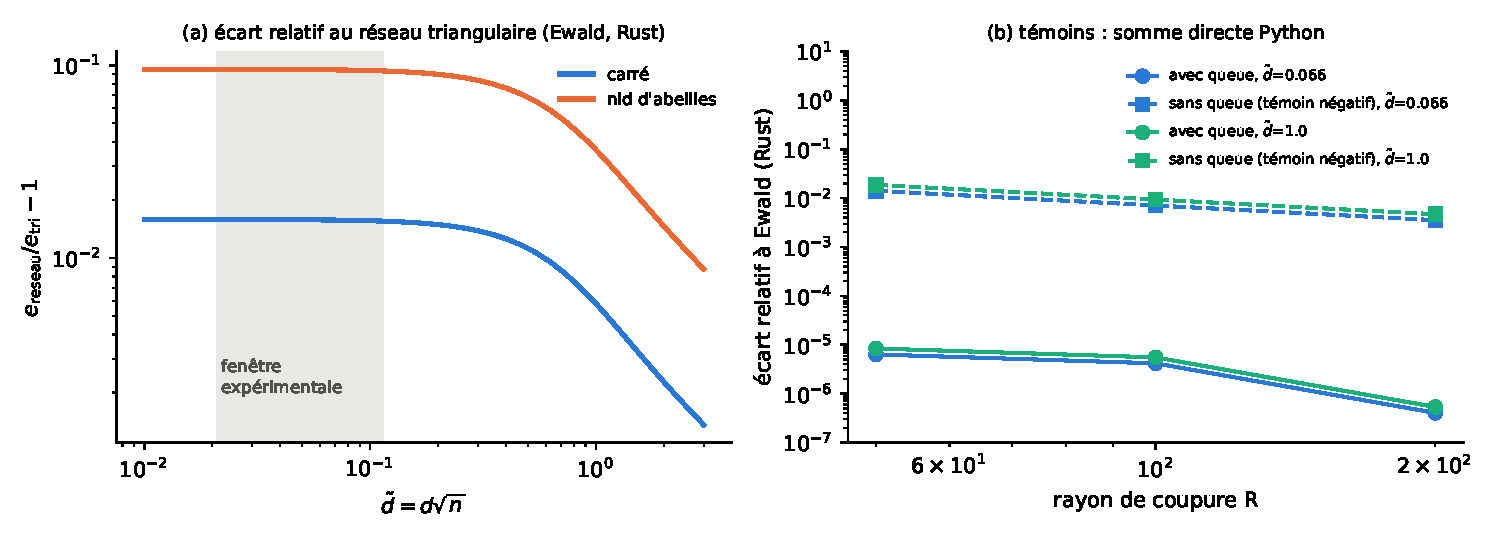
\includegraphics[width=\textwidth]{ch5_U1_dipolar.pdf}
\caption{U1 \tierX. (a) Écart relatif des réseaux carré et en nid d'abeilles au réseau triangulaire (énergies
d'Ewald exactes, rusty-SUNDIALS), en fonction de $\tilde d$. La bande grise est la fenêtre expérimentale déduite de
JARVIS-DFT. (b) Témoins : une somme directe en Python, \emph{avec} la queue uniforme exacte, converge vers la
valeur d'Ewald ; \emph{sans} la queue (témoin négatif), l'erreur reste de l'ordre de $10^{-2}$.}\label{ch5:fig:U1}
\end{figure}

\paragraph{Le résultat \tierX.} Sur toute la grille, les deux écarts restent positifs :
\begin{itemize}
\item $e_\mathrm{carre}/e_\mathrm{tri}-1$ décroît de $1{,}58\times10^{-2}$ à $1{,}36\times10^{-3}$ ;
\item l'écart du nid d'abeilles décroît de $9{,}53\times10^{-2}$ à $8{,}75\times10^{-3}$.
\end{itemize}
Converti en énergie (non écrantée, à diviser par $\varepsilon_r$), l'écart carré moins triangulaire vaut
$0{,}0014$, $0{,}044$ et $0{,}224$~meV par exciton aux trois densités. Ces valeurs sont interpolées sur la grille ;
l'article donnait $0{,}223$~meV au point de grille le plus proche. C'est de un à cinq ordres de grandeur sous la
profondeur des puits de moiré, \og des dizaines à 100~meV \fg{}~\cite{ch5:wang}. Dans l'étude publiée, aucun
des 21 compétiteurs relaxés par CVODE n'est passé sous le réseau triangulaire~\cite{ch2dip}.

\paragraph{Les témoins.}
\begin{itemize}
\item \emph{Positif.} Une somme directe Python indépendante, plus la queue exacte $2\pi/(\sqrt{R^2+\tilde
d^2}+R)$, retrouve la valeur d'Ewald de Rust. L'écart relatif est de $4{,}0\times10^{-7}$ à $\tilde d=0{,}066$ et
de $5{,}3\times10^{-7}$ à $\tilde d=1$, pour $R=200$. L'énergie d'Ewald ne dépend pas du paramètre de
découpage $\eta$ à mieux que $9{,}0\times10^{-15}$ près.
\item \emph{Négatif.} Sans la queue, la même somme se trompe de $3{,}5\times10^{-3}$ et $4{,}7\times10^{-3}$ à
$R=200$, et de $1{,}4\times10^{-2}$ à $R=50$.
\item \emph{Négatif.} Le script vérifie que $h_d(d^2)<0$ pour $d=0{,}5$, $1$ et $2$. Les réseaux carré et en nid
d'abeilles gardent une énergie plus haute en chacun des 41 points de la grille.
\end{itemize}
Nous avons aussi relancé, à part, deux relaxations de l'étude publiée à $\tilde d=0{,}066$ (commande
\texttt{dipolar\_crystal main <dossier> 0.066 1 0 1}, environ 8~minutes sur deux c\oe urs) :
\begin{itemize}
\item le départ uniforme \texttt{uniform\_00} finit à un écart relatif de $1{,}382373\times10^{-3}$, avec 4 défauts ;
\item la boîte incommensurable, témoin négatif, finit à $2{,}000407\times10^{-3}$, avec 8 défauts.
\end{itemize}
Ces deux valeurs sont celles de l'enregistrement, chiffre pour chiffre.

\paragraph{Ce que cela ne montre pas.}
\begin{itemize}
\item Le modèle est classique, à température nulle, avec des dipôles rigides et sans écrantage : pas de forme de
Rytova--Keldysh, pas de potentiel de moiré, pas d'énergie cinétique. Dans la fenêtre expérimentale, les vrais excitons
forment un gaz quantique, pas un cristal classique~\cite{ch5:wang}.
\item Le $d$ de JARVIS est un substitut : celui de deux empilements homogènes, et non celui d'une hétérobicouche. Le jeu
de données fixe l'échelle de $\tilde d$ ; il ne teste pas le théorème.
\item Aucune relaxation ne prouve l'optimalité : 21 essais ne couvrent pas l'infinité des configurations.
\end{itemize}

% =====================================================================================================
\section{U2 -- Cristaux de Yukawa plans : plasmas poussiéreux et colloïdes}\label{ch5:U2}

\paragraph{La question.} Dans un plasma poussiéreux de laboratoire, des micrograins chargés lévitent dans un plan.
Ils se repoussent par un potentiel coulombien écranté par les ions, $V(r)=Q^2e^{-r/\lambda_D}/r$. Des colloïdes
chargés en suspension se comportent de même. À densité fixée, quelle configuration minimise l'énergie ? On
observe des cristaux hexagonaux ; peut-on le démontrer dans ce modèle ?

\paragraph{Le théorème et son niveau.} Avec $t=r^2$ et $\kappa=\ell/\lambda_D$, où $\ell$ est la longueur
caractéristique de la densité, $g_\kappa(t)=e^{-\kappa\sqrt t}/\sqrt t$. La preuve humaine \tierC{} se fait en
trois étapes :
\begin{itemize}
\item $t\mapsto\sqrt t$ est une fonction de Bernstein et $x\mapsto e^{-\kappa x}$ est complètement monotone,
donc leur composée $e^{-\kappa\sqrt t}$ est complètement monotone (c'est la règle CM\,$\circ$\,Bernstein de la bibliothèque P3, doi:10.5281/zenodo.23653842) ;
\item $t^{-1/2}$ est complètement monotone ;
\item un produit de deux fonctions complètement monotones l'est encore (règle de Leibniz : chaque terme a le bon
signe).
\end{itemize}
Lean le vérifie \tierA{} (Lean 4.34.1), conditionnellement à l'amont :
\begin{leanbox}[: \texttt{formal\_cert/Autoresearch/Yukawa.lean} (énoncés)]
\begin{lstlisting}[language=Lean]
theorem yukawa_admissible {κ : ℝ} (hκ : 0 < κ) : AdmissiblePotential (g κ)
theorem triangular_yukawa_optimal {κ : ℝ} (hκ : 0 < κ) (C : Set Plane) (hC : LocallyFinite C)
    (hdens : DensityOne C) : latticeEnergy (g κ) ≤ energy (g κ) C
theorem latticeEnergy_yukawa_lt_top {κ : ℝ} (hκ : 0 < κ) : latticeEnergy (g κ) < ⊤
\end{lstlisting}
\end{leanbox}
Le module \texttt{YukawaMix.lean} étend le résultat à tout mélange fini $\sum_iw_ie^{-\kappa_ir}/r$ à poids
$w_i\ge0$. Le témoin négatif formel est le mélange signé $g_1-2g_2$ : il vaut $2e^{-1/2}-4e^{-1}\approx-0{,}2585$
en $t=\tfrac14$, donc il n'est pas admissible. Le théorème ne s'applique pas à lui, ce qui ne veut pas dire que
l'optimalité échoue. Article : doi:10.5281/zenodo.23646105~\cite{ch2yuk}.

\paragraph{Les données.} Le 2026-10-25, une recherche sur le Hub (\emph{dusty plasma}, \emph{complex plasma},
\emph{colloid}, \emph{yukawa}, \emph{wigner crystal}) n'a trouvé aucun jeu de positions de grains ou de
colloïdes~\cite{ch2yuk}. C'est une absence constatée par recherche, pas une preuve. Les conditions initiales
désordonnées viennent donc d'un tout autre domaine, la catalyse :
\begin{itemize}
\item identifiant \texttt{colabfit/OC20\_IS2RES\_val\_id}, licence CC-BY-4.0~\cite{ch5:oc20} ;
\item fichier \texttt{co/co\_10.parquet}, 142\,986\,687 octets ; son sha256 local est égal au hash LFS du Hub à la
révision \texttt{6a1dfef12aec878b4cda99edd54b16a6a254e135} ;
\item des structures d'adsorbats, tournées en 3D, projetées sur le plan, remises à l'échelle et filtrées par une
distance minimale.
\end{itemize}
Le script vérifie le sha256 et retrouve dans le fichier les identifiants de configuration OC20 listés dans
\texttt{provenance.json}. Ces données fournissent un \emph{désordre} d'aspect réaliste, rien de plus : des molécules
adsorbées sur un catalyseur n'ont rien à voir avec des grains chargés écrantés.

\paragraph{La méthode numérique.} Le module \texttt{exact.rs} de \texttt{qf-yukawa-crystal} a trois parties :
\begin{itemize}
\item des sommes de réseau du potentiel \emph{non tronqué}, avec une borne rigoureuse de la queue ;
\item une décomposition d'Ewald indépendante ;
\item une boîte périodique sommant toutes les images dans le rayon $R$, avec énergie, force et hessienne
analytiques.
\end{itemize}
La borne de queue repose sur les cellules de Voronoï : pour $V$ décroissant, la queue au-delà de $R$ vaut au plus
$(\pi/A)\bigl(1+\delta/(R-2\delta)\bigr)e^{-\kappa(R-2\delta)}/\kappa$. La relaxation (\texttt{exact-relax}) utilise
CVODE : BDF, jacobien égal à l'opposé de la hessienne, $\mathrm{rtol}=10^{-10}$, $\mathrm{atol}=10^{-12}$ et
tolérance de force $10^{-9}$. Chaque minimum est contrôlé par le spectre de la hessienne. Ce calcul corrige un
erratum publié : une version antérieure tronquait le potentiel à $r_c=8$ avec un décalage de force, et ce potentiel
tronqué n'est plus complètement monotone.

\paragraph{Le script.} \texttt{code/ch5\_U2\_yukawa.py SORTIE} :
\begin{enumerate}
\item il copie les conditions initiales dans une crate de travail ;
\item il lance \texttt{yukawa\_crystal exact-refs}, puis \texttt{exact-relax 2 1 0 0}. À $\kappa=2$, cela fait
trois relaxations d'environ 1 à 2~minutes chacune sur deux c\oe urs : un départ OC20, un départ uniforme et une
boîte incommensurable ;
\item il exécute les témoins et trace \texttt{figures/ch5\_U2\_yukawa.pdf}.
\end{enumerate}
L'option \texttt{--skip-relax} relit l'enregistrement au lieu de relancer les relaxations.

\begin{figure}[ht]\centering
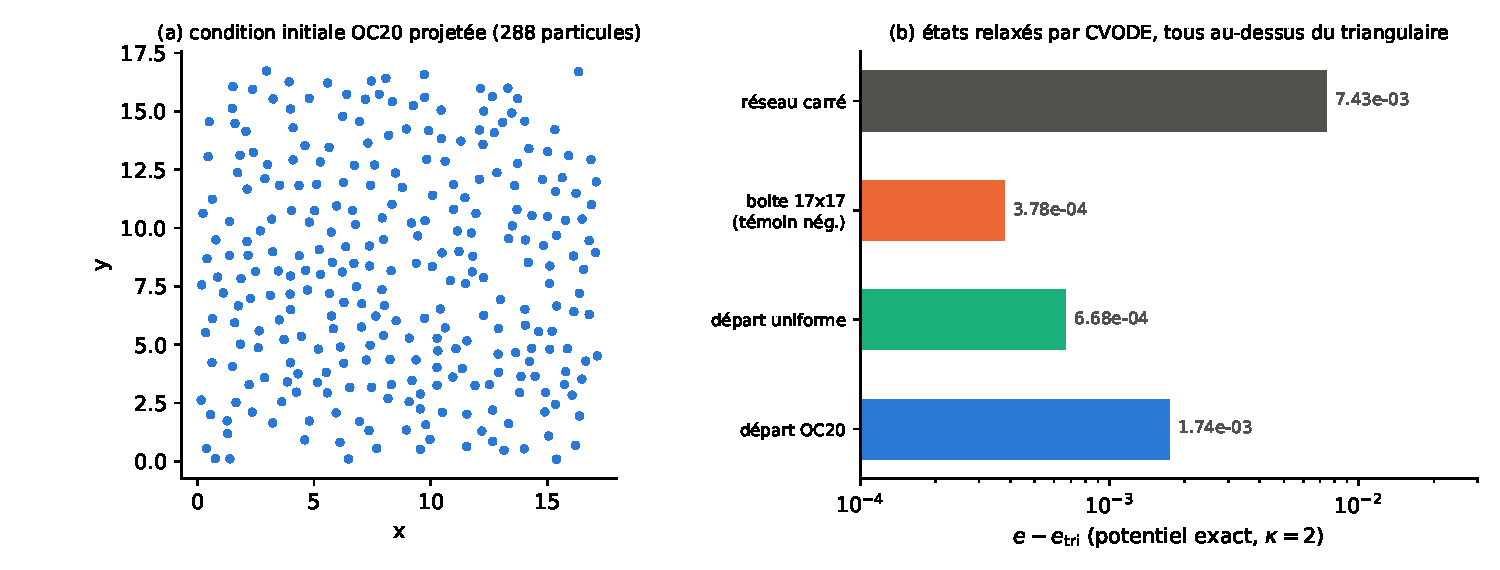
\includegraphics[width=\textwidth]{ch5_U2_yukawa.pdf}
\caption{U2 \tierX. (a) Condition initiale tirée d'OC20 (288 particules dans une boîte qui contient exactement le
réseau triangulaire). (b) Écart $e-e_\mathrm{tri}$ des états relaxés par CVODE sous le potentiel exact
($\kappa=2$), à comparer à l'écart du réseau carré. Aucun état n'est en dessous du réseau
triangulaire.}\label{ch5:fig:U2}
\end{figure}

\paragraph{Le résultat \tierX.} Énergies par particule à densité un, en convention $\tfrac12\sum$ :

\begin{center}\small
\begin{tabular}{lllll}\toprule
$\kappa$ & triangulaire (exact) & carré (exact) & écart & tronqué--exact (tri.)\\\midrule
1 & 1,6253213396063 & 1,6348554953172 & $9{,}534\times10^{-3}$ & $-1{,}771\times10^{-2}$\\
2 & 0,3935428489324 & 0,4009742487651 & $7{,}431\times10^{-3}$ & $-9{,}48\times10^{-6}$\\
\bottomrule\end{tabular}
\end{center}
La borne de queue vaut au plus $5{,}6\times10^{-17}$ ($\kappa=1$, $R=40$) et $1{,}2\times10^{-16}$ ($\kappa=2$,
$R=20$). Les trois relaxations à $\kappa=2$ convergent, sans mode négatif de la hessienne :
\begin{itemize}
\item départ OC20 : écart $1{,}742\times10^{-3}$, 24 défauts, 157 pas de CVODE ;
\item départ uniforme : écart $6{,}68\times10^{-4}$, 4 défauts ;
\item boîte incommensurable $17\times17$ : écart $3{,}78\times10^{-4}$, 4 défauts.
\end{itemize}
Dans l'étude complète, aucune des 24 étapes relaxées sous le potentiel exact n'est passée sous le réseau
triangulaire~\cite{ch2yuk}.

\paragraph{Les témoins.}
\begin{itemize}
\item \emph{Positifs.} Une somme directe Python du réseau retrouve les valeurs exactes de Rust à
$1{,}4\times10^{-16}$ près en relatif au plus (le seuil exigé est $10^{-12}$). Par ailleurs, la boîte périodique contenant le réseau parfait égale la somme
infinie à $2{,}2\times10^{-16}$ près.
\item \emph{Négatifs.} Les énergies tronquées à $r_c=8$ ratent la valeur exacte de bien plus que $10^{-9}$. La boîte
$17\times17$, qui ne peut pas contenir le réseau triangulaire, reste au-dessus. Le réseau carré parfait est un col
du potentiel exact, avec 72 modes négatifs à $\kappa=2$ et 64 à $\kappa=1$~\cite{ch2yuk}.
\end{itemize}

\paragraph{Ce que cela ne montre pas.}
\begin{itemize}
\item Les données OC20 ne contiennent aucune physique des plasmas : elles servent seulement de désordre initial.
\item Le potentiel $K_0(\kappa r)$, la fonction de Green de Debye--Hückel en 2D, n'est pas traité. Les mélanges à poids
négatifs, la température finie et l'unicité ne le sont pas non plus.
\item Le recuit n'a pas été refait avec le potentiel exact.
\end{itemize}

% =====================================================================================================
\section[U3 -- Hélium superfluide et test de Feynman--Bijl]{U3 -- Hélium superfluide : facteur de structure et test de Feynman--Bijl}\label{ch5:U3}

\paragraph{La question.} La diffraction de rayons X ou de neutrons mesure le facteur de structure statique $S(k)$
d'un liquide. Pour un gaz de Bose faiblement interagissant, la théorie de Bogoliubov prédit
$S_B(k)=\varepsilon_0(k)/\varepsilon_B(k)$, avec $\varepsilon_0=\hbar^2k^2/2m$. Peut-on dire, \emph{à partir de
$S(k)$ seul}, que l'hélium~4 superfluide n'est pas un gaz de Bogoliubov ?

\paragraph{Le théorème et son niveau.} Posons $k^*=2mc/\hbar$, où $c$ est la vitesse du son. On a alors
$S_B(k)=k/\sqrt{k^{*2}+k^2}$ et
\[S_B(k)\le\sqrt{\frac{k}{2k^*}},\qquad\text{avec égalité si et seulement si }k=k^* .\]
\begin{humanproof}
Les deux membres sont positifs ; on compare leurs carrés. $S_B^2\le k/2k^*$ équivaut à
$2k^*k\le k^{*2}+k^2$, c'est-à-dire à $(k-k^*)^2\ge0$.
\end{humanproof}
L'énoncé est de niveau \tierAs{}, dans l'environnement QuantumFluids (Lean v4.34.0-rc2 ; aucun rejeu \texttt{leanchecker} enregistré pour cet environnement), sous le nom
\lean{sBog_le_sqrt}. Les deux témoins sont vérifiés par le noyau : le test se déclenche sur la valeur libre $S=1$
pour tout $0<k<2k^*$ (\lean{free_S_one_violates}), et ne se déclenche jamais sur $S_B$. Le corollaire
\lean{not_bogoliubov_of_structure_factor} donne le \og test de diffraction \fg{} : si un $S$ mesuré dépasse
$\sqrt{k/2k^*}$, ce $S$ n'est pas le facteur de structure d'un gaz de Bogoliubov ayant cette vitesse du son.
L'argument de Feynman--Bijl relie $S$ à l'énergie d'excitation, $\varepsilon(k)\le\hbar^2k^2/(2mS(k))$. Son
c\oe ur à un mode est formalisé en Lean 4.34.1, l'identité de la règle de somme f étant prise comme
\emph{hypothèse}. Articles : doi:10.5281/zenodo.23646117~\cite{ch3-bsk} et
doi:10.5281/zenodo.23653846~\cite{ch3-fb}.

\paragraph{Les données (pas Hugging Face).} Aucun jeu de données de facteur de structure n'existe sur le Hub : les
recherches de ces deux articles n'en ont trouvé aucun. Nous utilisons la Table~14.1 de la compilation de Donnelly et
Barenghi~\cite{ch3-db}, dans son édition web (supposée, sans vérification, reproduire la table de 1998) :
\begin{itemize}
\item 99 points avec $Q>0$ : 49 points de rayons X (Robkoff--Hallock) et 50 points de neutrons (Svensson et al.) ;
\item des températures de 1,4 à 4~K, aucune barre d'erreur imprimée.
\end{itemize}
C'est une source secondaire de niveau \tierL{}. Le fichier extrait est
\url{papers/prog_superfluid_structure_factor/data/he4_Sk_donnelly_table14_1.csv}. On prend
$c=238{,}3\pm0{,}1$~m/s~\cite{ch3-godfrin}, d'où $k^*=3{,}00379$~\AA$^{-1}$ (entre 3,0025 et 3,0051).

\paragraph{La méthode.} Pour chaque point, le verdict est :
\begin{itemize}
\item \textsc{compatible} si $S\le\sqrt{Q/2k^*}$ ;
\item \textsc{réfuté} si $S-\sqrt{Q/2k^*}>\Delta$ ;
\item \textsc{indécis} sinon.
\end{itemize}
Le seuil $\Delta=0{,}082$ est l'écart entre les maxima des deux jeux de la table. Ce seuil a été fixé après coup, il
n'était pas préenregistré. Côté rusty-SUNDIALS, le module \texttt{linear\_response} de \texttt{qf-gpe2d} donne une
contre-épreuve : on excite le fondamental de Gross--Pitaevskii (grille $32\times32$, pas fractionnaire de Strang),
on mesure la fréquence de la réponse, et l'on en tire $\varepsilon_B(k)$ et $S(k)$.

\paragraph{Le script.} \texttt{code/ch5\_U3\_helium.py SORTIE [--gpe-json FICHIER]} applique le test et exécute les
témoins. Si on lui donne la sortie de l'exemple \texttt{bogoliubov\_dispersion} de \texttt{qf-gpe2d}, il trace aussi
la réponse linéaire.

\begin{figure}[ht]\centering
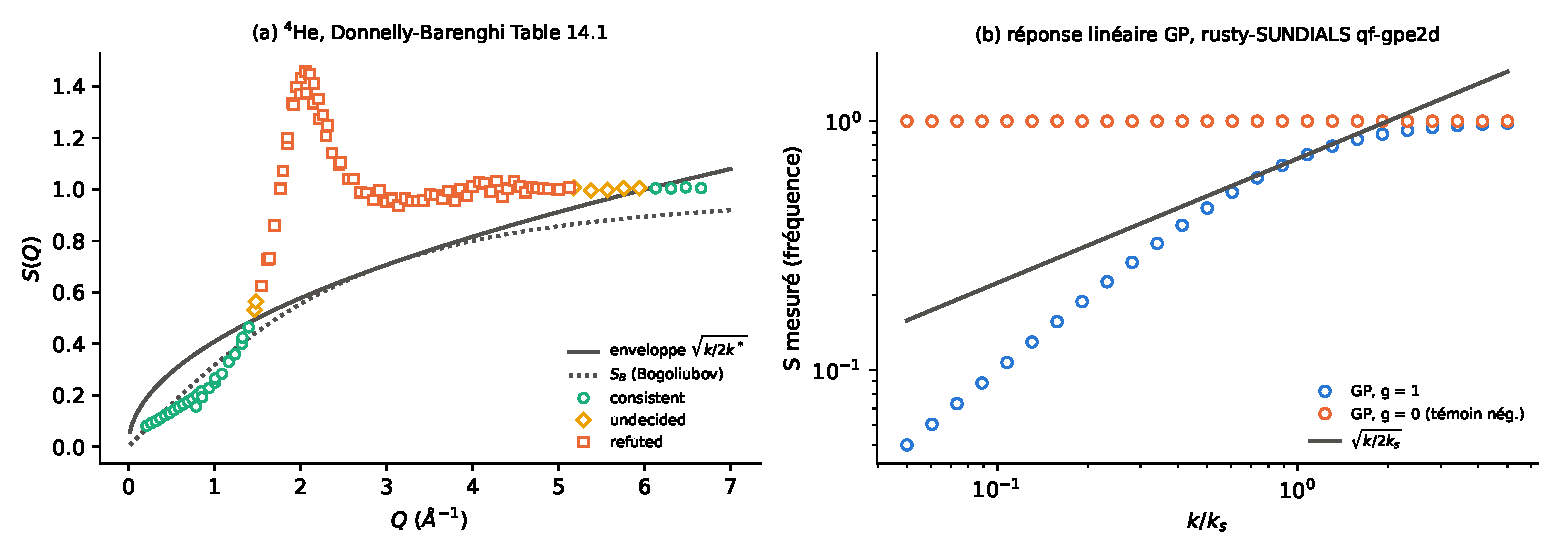
\includegraphics[width=\textwidth]{ch5_U3_helium.pdf}
\caption{U3. (a) $S(Q)$ de l'hélium~4 (Table~14.1, niveau~L) face à l'enveloppe $\sqrt{Q/2k^*}$ (trait plein) et à
$S_B$ (pointillé) ; la couleur donne le verdict (arithmétique, niveau~X). (b) Réponse linéaire de Gross--Pitaevskii
calculée par rusty-SUNDIALS \tierX{} : $S$ mesuré pour $g=1$ sous l'enveloppe, témoin $g=0$ ($S=1$) au-dessus pour
$k<2k_s$.}\label{ch5:fig:U3}
\end{figure}

\paragraph{Le résultat.} Sur les 99 points, 29 sont compatibles, 7 indécis et 63 réfutés. Les 21 points de la région
du pic et du roton ($1{,}7\le Q\le2{,}4$~\AA$^{-1}$) sont tous réfutés : $S$ y dépasse l'enveloppe d'un facteur
1,62 à 2,49. Les mesures de l'hélium~4 ne sont donc pas le $S$ d'un gaz de Bogoliubov de même vitesse du son. Ce
résultat de manuel est désormais une conséquence d'un énoncé vérifié et d'une table publiée.

Nous avons relancé l'exemple \texttt{bogoliubov\_dispersion} (10~min 24~s sur un c\oe ur), et sa sortie est
identique bit à bit à l'enregistrement. Dans cette réponse linéaire de Gross--Pitaevskii \tierX{} :
\begin{itemize}
\item la fréquence mesurée pour $g=1$ retrouve $\varepsilon_B$ à $4{,}1\times10^{-5}$ près en relatif ;
\item le $S$ mesuré reste sous l'enveloppe, puisque $\max(S/\sqrt{k/2k_s})-1=-1{,}4\times10^{-3}$ ;
\item le témoin $g=0$, un gaz libre où $S=1$, dépasse l'enveloppe aux 20 nombres d'onde du balayage tels que
$k<2k_s$.
\end{itemize}

\paragraph{Les témoins.}
\begin{itemize}
\item \emph{Positif.} $S_B$ ne déclenche le test en aucun des 99 points.
\item \emph{Négatif.} La valeur libre $S=1$ le déclenche en 95 points sur 95 avec $Q<2k^*$.
\end{itemize}
Les deux témoins sont aussi des théorèmes Lean.

\paragraph{Ce que cela ne montre pas.}
\begin{itemize}
\item La conclusion physique est conditionnelle \tierC{} : la table a été mesurée entre 1,4 et 4~K, et non à
$T=0$. Nous n'avons pas quantifié la variation du pic de $S$ avec la température.
\item Un point compatible n'est pas \emph{confirmé} \og Bogoliubov \fg{} : l'enveloppe n'est qu'une borne
supérieure, et aux petits $k$ elle a très peu de pouvoir de test.
\item Au-delà du pic, l'échec ressemble à celui du témoin $S=1$ : ce n'est plus la physique du roton.
\end{itemize}

% =====================================================================================================
\section[U4 -- Turbulence : borne d'enstrophie]{U4 -- Turbulence : borne d'enstrophie dans le modèle en couches \texorpdfstring{$\sigma=3$}{sigma=3}}\label{ch5:U4}

\paragraph{La question.} Les modèles en couches remplacent un champ de vitesse turbulent par une amplitude complexe
$v_n$ par octave de nombres d'onde, $k_n=2^n$, $n=0,\dots,N+1$. Les couches voisines échangent de l'énergie par un
terme quadratique. Ajoutons un terme dispersif $-i\omega_nv_n$ avec $\omega_n=Dk_n^3$ (\og $\sigma=3$ \fg). Peut-on
borner l'enstrophie $\Omega=\tfrac12\sum k_n^2|v_n|^2$, qui mesure les petites échelles, le long de \emph{toute}
trajectoire et pour \emph{toute} troncature $N$ ?

\paragraph{Le théorème et son niveau.} Le modèle conserve deux quantités :
\begin{itemize}
\item la \og masse \fg{} $S=\sum|v_n|^2=2E$ ;
\item l'invariant $H=\sum2^{-n}\omega_n|v_n|^2+\sum2^{-n}k_n\,\mathrm{Im}(\bar v_n^{\,2}v_{n+1})$, pour \emph{toute}
loi de dispersion réelle.
\end{itemize}
Pour $\omega_n=Dk_n^3$, la partie quadratique de $H$ vaut exactement $2D\Omega$. La partie cubique $C$ vérifie
$|C|\le S^{3/2}$.
\begin{humanproof}
Notons $H_3(0)$ la valeur de $H$ à l'instant $0$. Comme $H$ est conservé, $2D\Omega(t)=H_3(0)-C(t)$. Donc
$2D\Omega(t)\le H_3(0)+|C(t)|\le H_3(0)+S(t)^{3/2}$. Comme $S$ est conservé,
$2D\Omega(t)\le H_3(0)+(2E(0))^{3/2}$.
\end{humanproof}
Lean vérifie tout cela \tierAs{} (Lean v4.34.0-rc2, Mathlib du projet ; sans rejeu \texttt{leanchecker}) :
\begin{itemize}
\item l'identité de taux de $H$ le long du champ de vecteurs ;
\item la règle de dérivation en chaîne ;
\item la constance de $H$ et de $S$ sur $[0,T]$ ;
\item la borne \lean{enstrophy_bound_along_flow}, pour toute trajectoire sur $[0,T]$ et tout $N$.
\end{itemize}
L'énoncé suppose que la trajectoire existe et qu'elle est dérivable en chaque instant de $[0,T]$ : l'existence est
une \emph{hypothèse}, pas un théorème. Le niveau $N$ reste fixé. Article : doi:10.5281/zenodo.23646111~\cite{ch5:sigma3}.
\paragraph{Les données.} The Well~\cite{ch5:thewell} contient des simulations de fluides de grande taille. Nous
utilisons :
\begin{itemize}
\item identifiant : \url{polymathic-ai/turbulent_radiative_layer_2D} ;
\item révision \texttt{2ee7756575ff6f90981d0308cbcb6a2ab5995bdc}, licence CC-BY-4.0 selon la carte ;
\item le fichier\\ \url{data/test/turbulent_radiative_layer_tcool_0.32.hdf5},\\ sha256 \texttt{06cbd36c\dots f747},
vérifié par le script.
\end{itemize}
Ce sont des simulations Athena++ de l'équation d'Euler compressible 2D avec refroidissement radiatif.

Le spectre est construit ainsi, pour quatre instantanés développés (indices 25, 50, 75 et 100) :
\begin{enumerate}
\item on prend la FFT de la vitesse selon l'axe périodique $x$, sans le mode $k_x=0$ ;
\item on fait la moyenne en $y$ ;
\item on somme $k_x\in[2^n,2^{n+1})$ dans la couche $n=0,\dots,5$.
\end{enumerate}
Cette étape lit le HDF5 avec \texttt{h5py}, absent de l'environnement \texttt{.venv} d'AutoevolveAI : le script
relit donc le fichier \texttt{well\_amps.txt} que ces étapes ont produit. Les pentes de $\log_2$ des spectres valent
$-2{,}13$, $-1{,}56$, $-1{,}79$ et $-1{,}81$~\cite{ch5:sigma3}.

\paragraph{La méthode numérique.} Le module \texttt{sigma.rs} de \texttt{qf-shell-cascade} intègre le modèle avec CVODE :
\begin{itemize}
\item BDF, jacobien analytique, $\mathrm{atol}=10^{-3}\,\mathrm{rtol}$, $D=0{,}05$ ;
\item suprema pris aux points de pas internes de CVODE, sans interpolation.
\end{itemize}
Le programme \texttt{sigma3\_study full} enchaîne cinq blocs :
\begin{itemize}
\item un témoin positif, la convergence de la conservation avec la tolérance ;
\item un témoin négatif, un couplage perturbé ;
\item un balayage de troncatures $n_{\max}\le7$ ;
\item la comparaison $\sigma=2$ contre $\sigma=3$ sur des données concentrées dans la dernière couche ;
\item 24 trajectoires initialisées par les modules de The Well, avec deux tirages de phases aléatoires et
$n_{\max}=5,6,7$.
\end{itemize}

\paragraph{Le script.} \texttt{code/ch5\_U4\_shell.py SORTIE} lance \texttt{sigma3\_study full} (de 2,5 à 6~minutes
selon la charge de la machine), vérifie les critères et trace \texttt{figures/ch5\_U4\_shell.pdf}.

\begin{figure}[ht]\centering
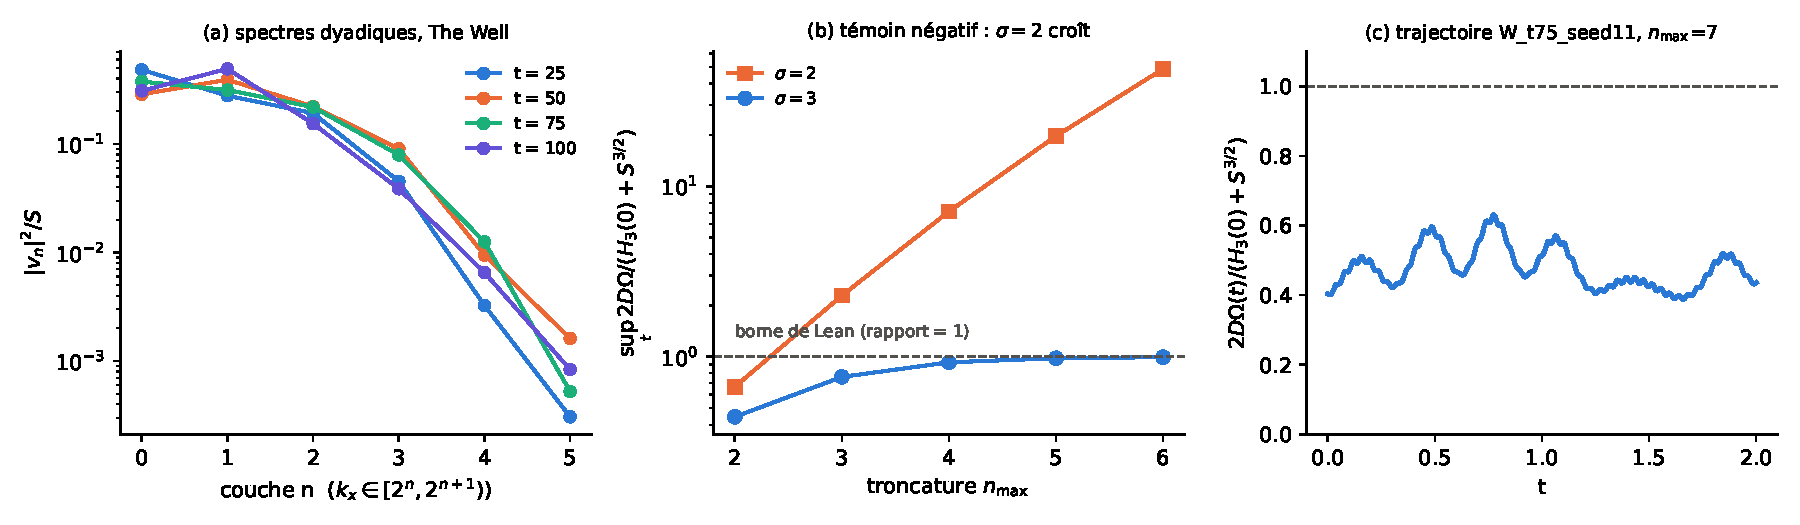
\includegraphics[width=\textwidth]{ch5_U4_shell.pdf}
\caption{U4 \tierX. (a) Spectres dyadiques de quatre instantanés de The Well, normalisés à $S=1$. (b) Rapport
$\sup_t2D\Omega/(H_3(0)+S^{3/2})$ sur des données concentrées dans la dernière couche : il reste sous 1 pour
$\sigma=3$ et croît avec $n_{\max}$ pour $\sigma=2$ (témoin négatif). (c) Le rapport le long de la trajectoire
initialisée par The Well qui s'approche le plus de la borne.}\label{ch5:fig:U4}
\end{figure}

\paragraph{Le résultat \tierX.} Les 17 trajectoires $\sigma=3$ du balayage et de la comparaison restent toutes sous la
borne. Le rapport $\sup_t2D\Omega(t)/(H_3(0)+S(0)^{3/2})$ vaut au plus 0,995 ; ce maximum est atteint sur des données
concentrées dans la dernière couche, où le rapport tend vers 1 quand $n_{\max}$ croît (0,444, 0,762, 0,928, 0,981
et 0,995 pour $n_{\max}=2,\dots,6$). Les 24 trajectoires initialisées par The Well restent aussi sous la borne, avec
un rapport d'au plus 0,631. Leurs dérives relatives sont au plus $2{,}4\times10^{-8}$ sur $S$ et $1{,}2\times10^{-6}$
sur $H$. Le fichier \texttt{sigma3\_study.json} recalculé est identique à l'enregistrement de
l'article~\cite{ch5:sigma3}, aux temps d'exécution près.

\paragraph{Les témoins.}
\begin{itemize}
\item \emph{Positif.} Avec le vrai couplage, la dérive de $H$ diminue avec la tolérance. Pour $n_{\max}=4$, elle
vaut $2{,}6\times10^{-5}$, $8{,}6\times10^{-7}$ puis $1{,}9\times10^{-8}$ pour
$\mathrm{rtol}=10^{-6},10^{-8},10^{-10}$.
\item \emph{Négatif.} Si l'on perturbe le couplage sortant de la couche~1 de $10^{-2}$, la dérive de $H$ reste
bloquée vers $2{,}3\times10^{-3}$ ($n_{\max}=4$) et $5{,}4\times10^{-3}$ ($n_{\max}=6$), quelle que soit la
tolérance. La conservation vient donc de la structure du modèle, pas de la précision du solveur.
\item \emph{Négatif.} Pour $\sigma=2$, la même inégalité n'a pas de démonstration, et le rapport vaut 0,667, 2,29,
7,11, 19,7 puis 48,8 pour $n_{\max}=2,\dots,6$. Il dépasse 1 dès $n_{\max}=3$ et croît plus vite qu'une
exponentielle de raison 2 sur cette plage (figure~\ref{ch5:fig:U4}b).
\end{itemize}

\paragraph{Ce que cela ne montre pas.}
\begin{itemize}
\item Les données de The Well donnent une forme de spectre réaliste, et rien d'autre. L'écoulement est compressible
et refroidi, il ne conserve pas l'énergie. Le spectre est unidimensionnel et ne porte pas de phases (elles sont
tirées au hasard).
\item Sur $T=2$, les couches supérieures, initialement vides, se remplissent à peine. Ces trajectoires ne sondent donc
pas la dépendance en $N$.
\item Il n'y a aucun énoncé en nombre infini de couches. L'uniformité en $N$ demande des données initiales dont
$\Omega(0)$ et $S(0)$ sont bornés uniformément en $N$ (corollaire de niveau C).
\item L'amortissement de BDF fait dériver $S$ vers le bas. Les marges observées dépassent largement ces dérives,
mais la simulation ne remplace pas le théorème.
\end{itemize}

% =====================================================================================================
\section{U5 -- Génétique : fixation d'une mutation}\label{ch5:U5}

\paragraph{La question.} Une population compte $N$ individus, dont $i$ portent une mutation de valeur sélective
relative $r$. Quelle est la probabilité que la mutation finisse par envahir toute la population (la
\emph{fixation}) ? Et que devient cette probabilité quand la population vit sur un graphe ?

\paragraph{Le modèle de Moran.} À chaque pas, un individu est choisi pour se reproduire avec une probabilité
proportionnelle à sa valeur sélective, et un individu tiré uniformément meurt. Le nombre de mutants est une chaîne de
naissance et de mort sur $\{0,\dots,N\}$. Ses probabilités de montée et de descente sont
\[p_i=\frac{ri}{ri+N-i}\cdot\frac{N-i}{N},\qquad q_i=\frac{N-i}{ri+N-i}\cdot\frac iN,\qquad\text{donc } p_i=r\,q_i .\]

\paragraph{Le théorème et son niveau.} Notons $\varphi_i$ la probabilité de fixation partant de $i$ mutants. L'équation
du premier pas donne $p_i(\varphi_{i+1}-\varphi_i)=q_i(\varphi_i-\varphi_{i-1})$, avec $\varphi_0=0$ et
$\varphi_N=1$.
\begin{humanproof}[Démonstration humaine (formule)]
Posons $\delta_i=\varphi_{i+1}-\varphi_i$. L'équation donne $\delta_i=\delta_{i-1}/r$, donc $\delta_i=r^{-i}\delta_0$
et $\varphi_i=\delta_0S_i$, où $S_i=\sum_{k<i}r^{-k}$. La condition $\varphi_N=1$ fixe
$\delta_0=1/S_N$. Pour $r\ne1$, on obtient
\[\varphi_i=\frac{S_i}{S_N}=\frac{1-r^{-i}}{1-r^{-N}} .\]
Pour $r=1$, on obtient $\varphi_i=i/N$.
\end{humanproof}
Le programme P7 vérifie davantage \tierA{} (Lean 4.34.1). Il montre la \emph{limite d'absorption},
$P^n(i,N)\to(1-r^{-i})/(1-r^{-N})$, et l'unicité : toute fonction harmonique à l'intérieur avec les valeurs $0$ et
$1$ au bord est $\varphi$. Le programme N4 démontre le théorème isotherme (naissance--mort) : sur un graphe
fortement connexe dont la matrice de remplacement est doublement stochastique, la fixation suit la même loi.
\begin{leanbox}[: \texttt{PopGen/MoranFixation.lean} et \texttt{EvoGraph/BirthDeath.lean} (énoncés)]
\begin{lstlisting}[language=Lean]
theorem moran_fixation_limit_closed {N : ℕ} {r : ℝ} (hN : 0 < N) (hr : 0 < r) (hr1 : r ≠ 1)
    (i : Fin (N + 1)) :
    Tendsto (fun n => kPow (moranP N r) n i (Fin.last N)) atTop
      (𝓝 ((1 - r⁻¹ ^ (i : ℕ)) / (1 - r⁻¹ ^ N)))
theorem moran_fixation_unique {N : ℕ} {r : ℝ} (hN : 0 < N) (hr : 0 < r) {g : Fin (N + 1) → ℝ}
    (hg : InteriorHarmonic (moranP N r) g) (g0 : g 0 = 0) (g1 : g (Fin.last N) = 1) :
    ∀ i, g i = moranFix N r i
theorem isothermal_fixation {W : Fin n → Fin n → ℝ} {r : ℝ} (hn : 0 < n) (hr : 0 < r)
    (hW : Isothermal W) (hsc : StronglyConnected W) (S : Finset (Fin n)) :
    Tendsto (fun t => sPow (bdK (fun _ => 1) W r) t S univ) atTop (𝓝 (moranFix n r S.card))
\end{lstlisting}
\end{leanbox}
Le théorème général d'absorption de P7 et la version à un seul mutant du théorème isotherme réapparaissent sous
les noms \lean{KAL} et \lean{ILENE} dans la section~\ref{ch5:acronymes}.

Le nombre de mutants sur un graphe n'est \emph{pas} une chaîne de Markov en général. Sur le 4-cycle, la probabilité de
montée d'un pas dépend de la configuration, $1/3$ contre $2/3$ à $r=2$. Ce qui est vrai, et prouvé, c'est le biais
\emph{par configuration} $P^+=r\,P^-$. Sur l'étoile à $n=3$ nœuds, qui n'est pas isotherme, les limites valent
$5/12$, $2/3$ et $7/12$, contre $4/7$ pour Moran. Articles : doi:10.5281/zenodo.23653850~\cite{ch4:P7} et
doi:10.5281/zenodo.23660071~\cite{ch4:N4}.

\paragraph{Les données : ce qu'elles illustrent, et ce qu'elles n'estiment pas.} Le dépôt Genetic de l'auteur
utilise les jeux \texttt{katarinagresova/Genomic\_Benchmarks\_*}~\cite{ch5:gb}. Nous en prenons un :
\begin{itemize}
\item identifiant \url{katarinagresova/Genomic_Benchmarks_demo_coding_vs_intergenomic_seqs}, révision
\texttt{85458172cab6cffad46cb172e64ca94780506ed6} ;
\item la partie test, \url{data/test-00000-of-00001-6fccc31405110e30.parquet}, 2\,456\,511 octets, sha256
\texttt{dfe13715\dots 9afe}.
\end{itemize}
La carte n'indique \emph{aucune} licence et ne dit pas ce que signifient les étiquettes 0 et 1. Nous ne
reproduisons que des statistiques agrégées, et la licence du paquet amont n'a pas été vérifiée.

Le script compte 25\,000 séquences, 12\,500 par étiquette, toutes de longueur 200, sans autre symbole que A, C, G et T.
La fraction de GC vaut 0,5381 pour l'étiquette~0 et 0,4004 pour l'étiquette~1 (figure~\ref{ch5:fig:U5}c).

C'est ce à quoi ressemble une donnée de séquence : une mutation ponctuelle y est le remplacement d'une lettre.
\textbf{Mais ce jeu n'estime aucune valeur sélective $r$}, et rien dans ce chapitre n'en tire une. Les valeurs de $r$
utilisées plus bas (0,8, 1, 1,2, 1,5 et 2) sont \emph{choisies}, pas mesurées.

\paragraph{La méthode numérique.} La crate \texttt{qf-popgen} écrit la chaîne absorbante comme une équation
différentielle linéaire, $\dot\pi=\pi(P-I)$ : c'est l'équation de Kolmogorov progressive de la chaîne uniformisée. Elle
l'intègre avec CVODE (BDF, jacobien exact, $\mathrm{rtol}=10^{-11}$, $\mathrm{atol}=10^{-15}$). Un
\emph{certificat d'absorption} refuse toute exécution douteuse, dans l'esprit « fail-closed » (qui refuse par défaut) : une exécution n'est
acceptée que si cinq conditions sont réunies :
\begin{itemize}
\item le noyau est stochastique et absorbant ;
\item la masse totale est conservée ;
\item aucune composante ne devient négative ;
\item la masse intérieure est tombée sous $10^{-9}$ ;
\item la masse en $N$ égale la cible à $10^{-8}$ près.
\end{itemize}
Le passage de l'équation différentielle au noyau à $n$ pas (un mélange de Poisson) n'est pas formalisé.

Enfin, \textbf{LeanFlow} certifie un nombre calculé. Sa fonction \texttt{lean.certify} accepte une affirmation sur des
encadrements rationnels et la traduit en un énoncé sur les entiers. La tactique \texttt{decide\_kernel}
(\lean{decide +kernel}) fait décider cet énoncé par le noyau, sans axiome supplémentaire. LeanFlow audite ensuite
\texttt{\#print axioms}, et un oracle exact en Python doit rendre le même verdict.

\paragraph{Le script.} \texttt{code/ch5\_U5\_fixation.py SORTIE} :
\begin{enumerate}
\item il télécharge le fichier à la révision épinglée, en vérifie l'empreinte et en tire les statistiques ;
\item il lance \texttt{fixation\_ode} ;
\item il compare les valeurs de CVODE aux fractions exactes ;
\item il soumet cinq affirmations à LeanFlow (Lean 4.34.1, cœur seul) ;
\item il trace \texttt{figures/ch5\_U5\_fixation.pdf}.
\end{enumerate}
Il dure une vingtaine de secondes.

\begin{figure}[ht]\centering
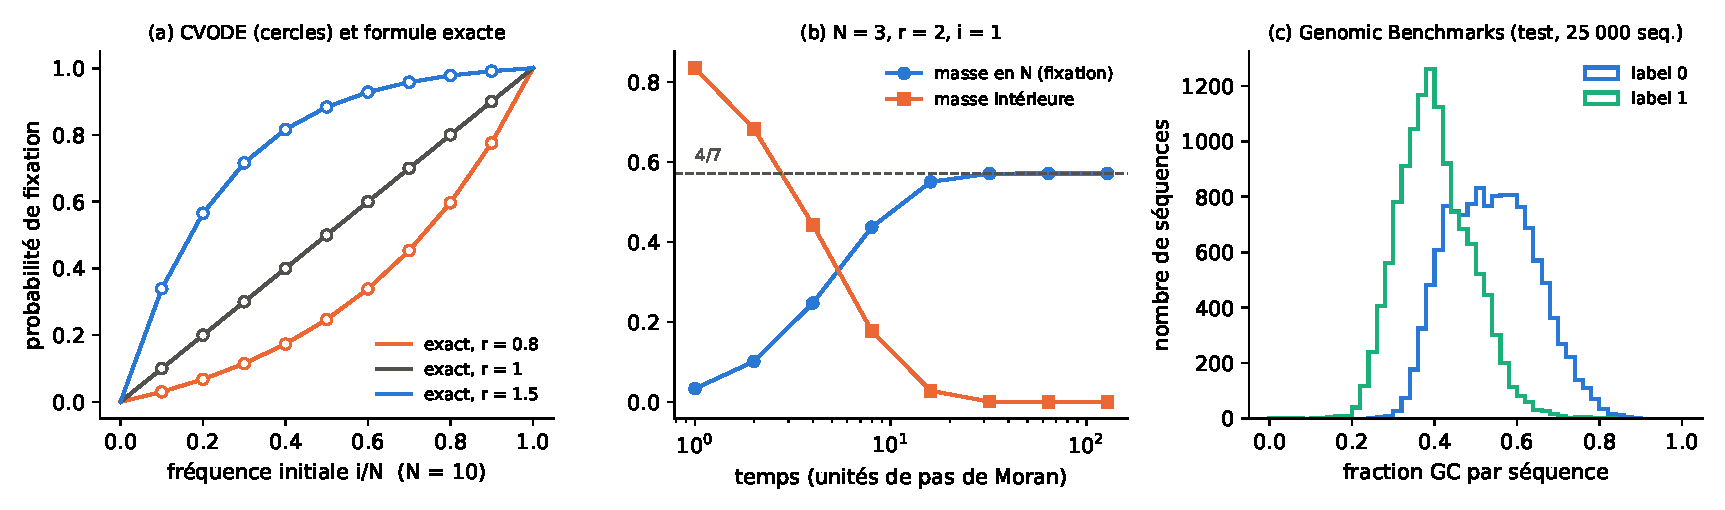
\includegraphics[width=\textwidth]{ch5_U5_fixation.pdf}
\caption{U5. (a) Probabilité de fixation pour $N=10$ : CVODE (cercles, \tierX) et formule exacte (traits), pour
$r=0{,}8$, $1$ et $1{,}5$. (b) Trajectoire de CVODE pour $N=3$, $r=2$, $i=1$ : la masse absorbée en $N$ tend vers
$4/7$, la masse intérieure s'éteint. (c) Fraction de GC des 25\,000 séquences de test de Genomic Benchmarks ; ce
jeu illustre des données de séquence et n'estime aucune valeur sélective.}\label{ch5:fig:U5}
\end{figure}

\paragraph{Le résultat.} \texttt{fixation\_ode} produit 115 lignes : 106 exécutions acceptées et 9 témoins négatifs
refusés, sans aucune exception. Sur les exécutions de Moran acceptées, l'écart maximal entre CVODE et la fraction
exacte $S_i/S_N$ est de $3{,}1\times10^{-10}$ \tierX.

Pour $N=3$, $r=2$, $i=1$, CVODE donne $0{,}5714285714284759$, soit un écart de $9{,}55\times10^{-14}$ à $4/7$.
LeanFlow certifie alors deux affirmations \tierA{} (sur l'énoncé arithmétique seulement, liste d'axiomes vide ; chaque affirmation est découpée par LeanFlow en propositions élémentaires) :
\begin{itemize}
\item \emph{proximité} : $4/7-10^{-11}<0{,}5714285714284759<4/7+10^{-11}$ ;
\item \emph{harmonicité} : le vecteur $(0,\tfrac47,\tfrac67,1)$ vérifie exactement les équations du premier pas de la
chaîne $N=3$, $r=2$, avec $p_1=\tfrac13$, $q_1=\tfrac16$, $p_2=\tfrac4{15}$ et $q_2=\tfrac2{15}$.
\end{itemize}
Voici une des quatre propositions engendrées, telle que le noyau l'a décidée :
\begin{lstlisting}[language=Lean]
-- harmonic at i=1
theorem cert_2 : (0 : Int) < ((((3 : Int) * (7 : Int)) * ((6 : Int) * (1 : Int))) * ((2 : Int) * (7 : Int))) ∧ ((((1 : Int) * (6 : Int)) * ((6 : Int) * (1 : Int)) + ((1 : Int) * (0 : Int)) * ((3 : Int) * (7 : Int))) * ((2 : Int) * (7 : Int)) + ((-1 : Int) * (4 : Int)) * (((3 : Int) * (7 : Int)) * ((6 : Int) * (1 : Int)))) * (1 : Int) = (0 : Int) * ((((3 : Int) * (7 : Int)) * ((6 : Int) * (1 : Int))) * ((2 : Int) * (7 : Int))) := by decide +kernel
\end{lstlisting}
LeanFlow n'audite que \texttt{\#print axioms}, qui peut être trompé ; nous avons donc complété la porte du
niveau~A pour ces deux certificats. Les deux sources engendrées ont été recompilées en \texttt{.olean} avec Lean
4.34.1 et rejouées par \texttt{leanchecker} : code de sortie~0 pour les deux. Le témoin de cette étape, un module
absent, sort avec le code~1. Une recherche de \texttt{skipKernelTC}, \texttt{addDecl}, \texttt{native\_decide} et
\texttt{implemented\_by} dans les deux sources ne trouve rien.

Combinée à \lean{moran_fixation_unique}, l'harmonicité dit que $4/7$ \emph{est} la probabilité de fixation de ce cas.
Ce raccord est un argument humain \tierC{} : il identifie l'énoncé entier de LeanFlow aux définitions
\lean{moranP} de P7. P7 contient d'ailleurs déjà \lean{cert_N3_r2_i1}, un certificat Lean écrit à la main pour la même
valeur.

\paragraph{Les témoins.}
\begin{itemize}
\item \emph{Négatifs, LeanFlow.} Trois affirmations fausses sont \emph{rejetées} (\texttt{false-statement}), et
\texttt{\#print axioms} y signale \lean{sorryAx} :
\begin{itemize}
\item la valeur neutre $1/3$ à la place de $4/7$ ;
\item une tolérance trop serrée, $10^{-14}$, plus petite que l'erreur réelle de $9{,}55\times10^{-14}$ ;
\item le vecteur neutre $(0,\tfrac13,\tfrac23,1)$, qui viole les deux équations intérieures.
\end{itemize}
\item \emph{Négatifs, CVODE.} Neuf témoins sont refusés, chacun pour la raison prévue :
\begin{itemize}
\item la formule à exposant inversé et la valeur neutre $i/N$ sous sélection (\texttt{ValueMismatch}, trois de
chaque) ;
\item le noyau identité, qui n'absorbe jamais, et un horizon trop court (\texttt{NotAbsorbed}) ;
\item une ligne dont la somme vaut $1{,}001$ (\texttt{InvalidKernel}).
\end{itemize}
\item \emph{Positifs.} Les cas $N=2$ et $N=3$ à $r=2$ retrouvent $2/3$, $4/7$ et $6/7$, et le cas neutre retrouve $i/N$.
\end{itemize}

\paragraph{Ce que cela ne montre pas.}
\begin{itemize}
\item Le jeu Genomic Benchmarks n'estime ni $r$, ni $N$, ni aucun paramètre de dynamique des populations. Son rôle
est pédagogique.
\item Le certificat LeanFlow porte sur l'arithmétique des nombres énoncés, pas sur la justesse de CVODE.
\item Le modèle de Moran suppose une taille constante, un seul locus et un $r$ constant. Le théorème isotherme est
prouvé dans le sens \og suffisant \fg{} seulement, pour la règle naissance--mort ; la réciproque et la règle
mort--naissance ne sont pas démontrées.
\end{itemize}

% =====================================================================================================
\section{Bilan : ce que les cinq cas enseignent}\label{ch5:bilan}

\begin{table}[ht]\centering\small
\caption{Témoins exécutés pour ce chapitre (sorties des scripts du 2026-10-26).}\label{ch5:tab:temoins}
\begin{tabular}{p{1.4cm}p{6.2cm}p{6.2cm}}\toprule
cas & témoin positif (doit réussir) & témoin négatif (doit échouer)\\\midrule
U1 & somme directe Python $+$ queue exacte : $4\times10^{-7}$ de l'Ewald Rust ($R=200$) &
sans la queue : erreur $3{,}5\times10^{-3}$ ; $h_d(d^2)<0$ ; boîte incommensurable au-dessus\\
U2 & somme directe Python : $\le1{,}4\times10^{-16}$ de Rust &
énergies tronquées à $r_c=8$ : erreur $\ge9{,}4\times10^{-6}$ ; boîte $17\times17$ au-dessus\\
U3 & $S_B$ ne déclenche jamais le test (0 sur 99) ; GP $g=1$ sous l'enveloppe &
$S=1$ le déclenche (95 sur 95) ; GP $g=0$ au-dessus (20 sur 20)\\
U4 & dérive de $H$ divisée par $\approx10^3$ quand rtol passe de $10^{-6}$ à $10^{-10}$ &
couplage perturbé : dérive bloquée vers $2$--$5\times10^{-3}$ ; $\sigma=2$ dépasse la borne\\
U5 & 106 exécutions acceptées ; deux certificats LeanFlow \texttt{ok} &
9 témoins CVODE refusés ; 3 affirmations LeanFlow rejetées\\
\bottomrule\end{tabular}
\end{table}

Trois leçons se dégagent des cinq cas.

\paragraph{Une donnée réelle n'est pas une preuve.} Aucun des cinq jeux de données ne teste un théorème de niveau~A.
Chacun a un rôle plus modeste, mais réel :
\begin{itemize}
\item JARVIS-DFT fixe l'échelle physique $\tilde d$ ;
\item OC20 fournit un désordre initial ;
\item la table de Donnelly et Barenghi \emph{réfute} une hypothèse de modélisation (\og l'hélium est un gaz de
Bogoliubov \fg) ;
\item The Well donne une forme de spectre ;
\item Genomic Benchmarks montre à quoi ressemble une séquence.
\end{itemize}
Le cas U3 est le seul où les données disent quelque chose de physique. Encore est-ce \emph{grâce} au théorème : la
réfutation n'a de sens que parce que l'enveloppe est démontrée.

\paragraph{Le désaccord est plus instructif que l'accord.} Un accord entre CVODE et une formule exacte, à
$3\times10^{-10}$ près (U5) ou à $10^{-16}$ près (U2), rassure sur le code, mais il ne dit rien du modèle. Ce sont
les témoins négatifs qui donnent leur valeur aux témoins positifs :
\begin{itemize}
\item en U2, une troncature innocente change l'énergie de $1{,}8\times10^{-2}$, deux fois l'écart entre carré et
triangulaire ;
\item en U4, un couplage perturbé de 1\,\% détruit une conservation qu'aucune précision ne restaure ;
\item en U5, une tolérance de $10^{-14}$ est rejetée parce que l'erreur réelle vaut $9{,}55\times10^{-14}$.
\end{itemize}

\paragraph{Chaque outil a sa portée.} Les trois outils se partagent le travail :
\begin{itemize}
\item Lean vérifie des énoncés sur des définitions ;
\item rusty-SUNDIALS calcule en virgule flottante ;
\item LeanFlow fait le pont, en certifiant qu'un nombre \emph{énoncé} vérifie une relation exacte.
\end{itemize}
Aucun des trois ne dit que le modèle décrit la nature. Chaque section se termine donc par \og ce que cela ne
montre pas \fg{}, et cette rubrique compte autant que le résultat.

% =====================================================================================================
\section{Les acronymes cachés}\label{ch5:acronymes}

Quelques théorèmes de ce livre portent, dans le code Lean, un second nom fait d'initiales. Ces noms ne
prouvent rien de nouveau : ce sont des ré-exportations de résultats déjà vérifiés par le noyau, chacune accompagnée
d'un rétro-acronyme dans sa documentation. Ils sont rassemblés dans
le fichier \texttt{Acronymes.lean} de \texttt{formal\_cert/Programmes/}, dont voici la liste.

\IfFileExists{acronymes_listing.tex}{% Generated from formal_cert/Programmes/Famille/Acronymes.lean (verbatim copy); do not edit by hand.
% Requires the book preamble (listings + \lstdefinelanguage{Lean} in main.tex).
\begin{lstlisting}[language=Lean,literate={ℝ}{{$\mathbb{R}$}}1 {ℤ}{{$\mathbb{Z}$}}1 {ℕ}{{$\mathbb{N}$}}1 {≤}{{$\le$}}1 {≥}{{$\ge$}}1 {≠}{{$\ne$}}1
  {→}{{$\to$}}1 {↔}{{$\leftrightarrow$}}1 {∀}{{$\forall$}}1 {∃}{{$\exists$}}1 {∧}{{$\wedge$}}1 {∨}{{$\vee$}}1
  {¬}{{$\neg$}}1 {⊤}{{$\top$}}1 {∈}{{$\in$}}1 {∉}{{$\notin$}}1 {∩}{{$\cap$}}1 {⁻¹}{{$^{-1}$}}1 {√}{{$\surd$}}1
  {π}{{$\pi$}}1 {ρ}{{$\rho$}}1 {κ}{{$\kappa$}}1 {α}{{$\alpha$}}1 {δ}{{$\delta$}}1 {ε}{{$\varepsilon$}}1 {σ}{{$\sigma$}}1
  {•}{{$\bullet$}}1 {∑}{{$\sum$}}1 {²}{{$^2$}}1 {₀}{{$_0$}}1 {₁}{{$_1$}}1 {₂}{{$_2$}}1 {‖}{{$\|$}}1 {⟨}{{$\langle$}}1 {⟩}{{$\rangle$}}1
  {𝓝}{{$\mathcal{N}$}}1 {∞}{{$\infty$}}1 {≥}{{$\ge$}}1 {×}{{$\times$}}1 {·}{{$\cdot$}}1 {∘}{{$\circ$}}1 {∖}{{$\setminus$}}1
  {ψ}{{$\psi$}}1 {φ}{{$\varphi$}}1 {λ}{{$\lambda$}}1 {μ}{{$\mu$}}1 {θ}{{$\theta$}}1 {Λ}{{$\Lambda$}}1 {∂}{{$\partial$}}1
  {—}{{---}}1 {–}{{--}}1 {é}{{\'e}}1 {ö}{{\"o}}1 {’}{{'}}1 {∫}{{$\int$}}1 {ι}{{$\iota$}}1]
import Triangular.AnyDensity
import Programmes.PopGen.Absorption
import Programmes.EvoGraph.BirthDeath
import Autoresearch.KeldyshCM
import Programmes.PopGen.Price

/-!
# Acronymes : cinq ré-exportations sous des noms courts

Each theorem below is a **re-export** of a result that is already kernel-checked elsewhere in
`formal_cert/`. The statement is copied verbatim from the source theorem and the proof is the source
theorem applied to its arguments; nothing new is proved here. The `example`s after each theorem check,
by `rfl`, that the re-exported constant has exactly the type of its source (same statement, not a
weaker or stronger one).

Each name is an acronym; its docstring gives the backronym.

| name      | source                                                     |
|-----------|------------------------------------------------------------|
| `ALIX`    | `TriangularDensity.triangular_optimal_any_density`         |
| `KAL`     | `ProgPopGen.fixation_limit`                                |
| `ILENE`   | `EvoGraph.isothermal_fixation_single`                      |
| `ALEXIS`  | `AutoresearchKeldysh.laplace_admissible`                   |
| `AURELIA` | `ProgPopGen.Price.fisher_haploid_nondecreasing`            |

`ALIX` rests on upstream openai/math `universal_energy_minimum` (AI-generated, not peer reviewed);
everything is conditional on the fidelity of the definitions it uses.
-/

namespace Acronymes

section Lattice

open OAI.AtomicTriangular TriangularDensity Filter Topology Set
open scoped Pointwise

/-- **A** **L**attice **I**s e**X**tremal.

At every density `ρ > 0` the rescaled triangular lattice `ρ^{-1/2} A` is locally finite, has density
`ρ`, and its lower energy is `≤` that of every locally finite density-`ρ` configuration, for every
admissible (completely monotone in `r²`) potential `h`. Re-export of
`TriangularDensity.triangular_optimal_any_density` (conditional on upstream). -/
theorem ALIX (h : ℝ → ℝ) (hh : AdmissiblePotential h) {ρ : ℝ} (hρ : 0 < ρ) :
    LocallyFinite ((Real.sqrt ρ)⁻¹ • A) ∧ DensityRho ρ ((Real.sqrt ρ)⁻¹ • A) ∧
      ∀ C : Set Plane, LocallyFinite C → DensityRho ρ C → energy h ((Real.sqrt ρ)⁻¹ • A) ≤ energy h C :=
  triangular_optimal_any_density h hh hρ

example : @ALIX = @triangular_optimal_any_density := rfl

end Lattice

section Absorption

open Filter Topology ProgPopGen

/-- **K**olmogorov **A**bsorption **L**imit.

For a stochastic kernel on `{0,...,N}` with absorbing ends, whose `n`-step kernel is the
Chapman–Kolmogorov power `kPow P n`: if `h` is interior-harmonic with `h 0 = 0`, `h N = 1` and the
one-step variance of `h` is positive at every interior state, then `P^n(i,N) → h i` and
`P^n(i,0) → 1 - h i`. Re-export of `ProgPopGen.fixation_limit`. -/
theorem KAL {N : ℕ} {P : Fin (N + 1) → Fin (N + 1) → ℝ} (hP : AbsorbingChain P) (hN : 0 < N)
    {h : Fin (N + 1) → ℝ} (hh : InteriorHarmonic P h) (h0 : h 0 = 0) (h1 : h (Fin.last N) = 1)
    (hvar : ∀ k : Fin (N + 1), 0 < (k : ℕ) → (k : ℕ) < N → 0 < ∑ j, P k j * (h j - h k) ^ 2)
    (i : Fin (N + 1)) :
    Tendsto (fun n => kPow P n i (Fin.last N)) atTop (𝓝 (h i)) ∧
    Tendsto (fun n => kPow P n i 0) atTop (𝓝 (1 - h i)) :=
  fixation_limit hP hN hh h0 h1 hvar i

example : @KAL = @fixation_limit := rfl

end Absorption

section Isothermal

open Finset Filter Topology EvoGraph

/-- **I**sothermal **L**aw: **E**very **N**ode **E**quivalent.

Birth–death updating with uniform selection on a strongly connected isothermal graph (`W` doubly
stochastic): a single mutant of fitness `r ≠ 1` placed at *any* node `v` fixes with limiting
probability `(1 - r⁻¹)/(1 - r^(-n))`, the same for every node and equal to Moran's value.
Re-export of `EvoGraph.isothermal_fixation_single`. -/
theorem ILENE {n : ℕ} {W : Fin n → Fin n → ℝ} {r : ℝ} (hn : 0 < n) (hr : 0 < r)
    (hr1 : r ≠ 1) (hW : Isothermal W) (hsc : StronglyConnected W) (v : Fin n) :
    Tendsto (fun t => sPow (bdK (fun _ => 1) W r) t {v} univ) atTop
      (𝓝 ((1 - r⁻¹) / (1 - r⁻¹ ^ n))) :=
  isothermal_fixation_single hn hr hr1 hW hsc v

example : @ILENE = @isothermal_fixation_single := rfl

end Isothermal

section Laplace

open MeasureTheory OAI.AtomicTriangular AutoresearchKeldysh

/-- **A**veraged **L**aplace **EX**ponentials **I**nherit **S**igns.

A positive mixture of decaying exponentials `fun t => ∫ e^{-t k(x)} m(x) dμ(x)` (with `k, m ≥ 0` and all
moments `∫ k^n e^{-c k} m dμ` finite for `c > 0`) is `AdmissiblePotential`: `C^∞` on `(0, ∞)`,
nonnegative, with alternating signs `(-1)^r g^{(r)} ≥ 0`, each exponential's signs passing to the
average. Re-export of `AutoresearchKeldysh.laplace_admissible`. -/
theorem ALEXIS {α : Type*} [MeasurableSpace α] {μ : Measure α} {k m : α → ℝ}
    (h : MixtureData μ k m) :
    AdmissiblePotential (fun t => ∫ x, Real.exp (-(t * k x)) * m x ∂μ) :=
  laplace_admissible h

example : @ALEXIS.{0} = @laplace_admissible.{0} := rfl

end Laplace

section Fisher

open ProgPopGen.Price

/-- **A**verage **U**nder **R**eplication: **E**volution **L**ifts **I**t, **A**lways.

Haploid selection with constant type fitnesses and no transmission bias, nonnegative abundances,
positive total abundance and positive mean fitness: the mean fitness does not decrease,
`wbar ≤ wbar'`. This is a special case of Fisher's fundamental theorem (haploid types, constant
fitnesses, no transmission bias), obtained from the exact identity `wbar' - wbar = Var(w)/wbar`
derived from the Price equation. Re-export of `ProgPopGen.Price.fisher_haploid_nondecreasing`. -/
theorem AURELIA {ι : Type*} (s : Finset ι) (n w : ι → ℝ)
    (hn : ∀ i ∈ s, 0 ≤ n i) (hN : 0 < ∑ i ∈ s, n i) (hW : 0 < ∑ i ∈ s, n i * w i) :
    wmean s n w ≤ wbarNext s n w :=
  fisher_haploid_nondecreasing s n w hn hN hW

example : @AURELIA.{0} = @fisher_haploid_nondecreasing.{0} := rfl

end Fisher

end Acronymes

#print axioms Acronymes.ALIX
#print axioms Acronymes.KAL
#print axioms Acronymes.ILENE
#print axioms Acronymes.ALEXIS
#print axioms Acronymes.AURELIA
\end{lstlisting}
}{}

% =====================================================================================================
\section{Exercices}\label{ch5:exercices}
Les exercices marqués (S) demandent d'exécuter un script ; prévoyez au plus deux c\oe urs, par exemple avec
\texttt{taskset -c 6,7}.

\begin{exercise}[U1, calcul]\label{ch5:ex:hd}
\begin{enumerate}
\item Montrer que $h_d(t)=t^{-1/2}-2(t+d^2)^{-1/2}$ vérifie $h_d(d^2)=(1-\sqrt2)/d$. En déduire que $h_d$ n'est
pas complètement monotone.
\item Avec $a=t^{-1/2}$ et $b=(t+d^2)^{-1/2}$, établir $(a-b)(a+b)=d^2a^2b^2$, puis $g_d(t)\le d^2t^{-3/2}$.
Pourquoi cette inégalité garantit-elle que \lean{latticeEnergy (g d)} est fini ?
\end{enumerate}
\end{exercise}

\begin{exercise}[U1, (S)]\label{ch5:ex:U1}
Exécutez \texttt{ch5\_U1\_dipolar.py}.
\begin{enumerate}
\item Vérifiez dans le JSON que $\tilde d=0{,}0660$ à $n=10^{12}$~cm$^{-2}$.
\item Ajoutez la densité $n=5\times10^{11}$~cm$^{-2}$ et donnez l'écart carré moins triangulaire en meV pour
$\varepsilon_r=4$.
\item Remplacez la queue exacte par $0$ pour $R=400$. L'erreur est-elle divisée par deux par rapport à $R=200$ ?
Expliquez-le avec la formule de la queue.
\end{enumerate}
\end{exercise}

\begin{exercise}[U2, calcul]\label{ch5:ex:U2a}
Vérifier à la main que $g_1-2g_2$ est négatif en $t=\tfrac14$. Montrer ensuite qu'un mélange
$\sum_iw_ie^{-\kappa_i\sqrt t}/\sqrt t$ à poids positifs est complètement monotone, en admettant le cas d'un seul
terme.
\end{exercise}

\begin{exercise}[U2, (S)]\label{ch5:ex:U2b}
Dans \texttt{exact\_refs.jsonl}, produit par le script, les lignes \texttt{"kind":"sweep"} donnent l'erreur des
énergies tronquées (\texttt{sf\_err}) en fonction de $r_c$.
\begin{enumerate}
\item Tracez $|\texttt{sf\_err}|$ à $\kappa=1$. À partir de quel $r_c$ devient-elle plus petite que l'écart carré moins
triangulaire, $9{,}5\times10^{-3}$ ?
\item Comparez avec la borne de queue de Voronoï.
\end{enumerate}
\end{exercise}

\begin{exercise}[U3, démonstration]\label{ch5:ex:U3a}
\begin{enumerate}
\item Montrer que $S_B(k)=\varepsilon_0/\varepsilon_B$ avec $\varepsilon_B=\sqrt{\varepsilon_0(\varepsilon_0+2gn)}$
s'écrit $k/\sqrt{k^{*2}+k^2}$, où $k^*=2mc/\hbar$ et $mc^2=gn$.
\item Établir l'enveloppe $S_B\le\sqrt{k/2k^*}$ et son cas d'égalité.
\item Montrer que $S=1$ dépasse l'enveloppe pour tout $0<k<2k^*$.
\end{enumerate}
\end{exercise}

\begin{exercise}[U3, (S)]\label{ch5:ex:U3b}
Modifiez \texttt{ch5\_U3\_helium.py} pour utiliser $c=238{,}2$ puis $238{,}4$~m/s. Les décomptes
29\,/\,7\,/\,63 changent-ils ? Recommencez avec $\Delta=0{,}04$. Quelle part du résultat dépend du seuil fixé après
coup ?
\end{exercise}

\begin{exercise}[U4, démonstration et (S)]\label{ch5:ex:U4}
\begin{enumerate}
\item Pour $\omega_n=Dk_n^3$, vérifier que $\sum2^{-n}\omega_n|v_n|^2=2D\Omega$.
\item En admettant la conservation de $H$ et de $S$, démontrer $2D\Omega(t)\le H_3(0)+(2E(0))^{3/2}$.
\item Lancez \texttt{sigma3\_study probe 6 3 0.05 0.5 1e-10}, puis \texttt{probe 6 2 0.05 0.5 1e-10}. Comparez les
champs \texttt{sup\_ratio}. Lequel des deux modèles la borne de Lean ne couvre-t-elle pas, et pourquoi ?
\end{enumerate}
\end{exercise}

\begin{exercise}[U5, calcul]\label{ch5:ex:U5a}
\begin{enumerate}
\item Calculer exactement $\varphi_1$ pour $N=10$ et $r=3/2$. Comparer avec la valeur de CVODE,
$0{,}33921585523416337$, imprimée dans \texttt{results.jsonl}.
\item Montrer que $p_i=r\,q_i$ et en déduire la formule $\varphi_i=S_i/S_N$.
\item Pour une population neutre ($r=1$), interpréter $\varphi_i=i/N$.
\end{enumerate}
\end{exercise}

\begin{exercise}[U5, LeanFlow, (S)]\label{ch5:ex:U5b}
En vous inspirant de la fonction \texttt{harmonic} du script, écrivez l'affirmation LeanFlow qui certifie que
$(\varphi_0,\dots,\varphi_{10})$ est harmonique pour la chaîne de Moran $N=10$, $r=3/2$.
\begin{enumerate}
\item Soumettez-la : le statut doit être \texttt{ok} et la liste d'axiomes vide.
\item Changez une seule valeur $\varphi_5$ d'une unité sur $10^{12}$ et vérifiez que trois assertions exactement sont
rejetées. Pourquoi trois ?
\end{enumerate}
\end{exercise}

\begin{exercise}[U5, données, (S)]\label{ch5:ex:U5c}
\begin{enumerate}
\item Téléchargez la partie \emph{train} du même jeu, à la même révision, et vérifiez qu'elle compte 75\,000 séquences,
comme l'annonce la carte.
\item Calculez la fraction de GC par étiquette.
\item Rédigez trois phrases qui expliquent pourquoi cette différence de composition ne fournit pas de valeur sélective
$r$ pour le modèle de Moran.
\end{enumerate}
\end{exercise}

\begin{exercise}[Témoins, (S)]\label{ch5:ex:temoins}
Choisissez un des cinq scripts et cassez volontairement un témoin positif. Par exemple, dans
\texttt{ch5\_U1\_dipolar.py}, oubliez le facteur $\tfrac12$ de la somme directe. Vérifiez que le script sort avec le
code~1. Expliquez pourquoi un script qui accepterait cette erreur ne testerait rien.
\end{exercise}

\label{ch5:fin}
